\documentclass{thesis}
\usepackage{graphicx}
%\usepackage[dvipdfmx]{graphicx}
\usepackage[dvipdfmx]{color}
\usepackage{float}
\usepackage{listings}
\usepackage{jvlisting} %日本語のコメントアウトをする場合jvlisting(もしくはjlisting)が必要
\usepackage{amsmath}
\usepackage{mathtools}
\usepackage{stmaryrd} % \llparenthesis & rrparenthesis
\usepackage[dvipsnames]{xcolor}
\usepackage[hyphens]{url}
\allowdisplaybreaks
%ここからソースコードの表示に関する設定
\lstset{
  basicstyle={\ttfamily},
  identifierstyle={\small},
  commentstyle={\smallitshape},
  keywordstyle={\small\bfseries},
  ndkeywordstyle={\small},
  stringstyle={\small\ttfamily},
  frame={tb},
  breaklines=true,
  columns=[l]{fullflexible},
  numbers=left,
  xrightmargin=0zw,
  xleftmargin=3zw,
  captionpos=b,
  numberstyle={\scriptsize},
  stepnumber=1,
  numbersep=1zw,
  lineskip=-0.5ex,
  moredelim=**[is][\color{red}]{!}{!} 
}
%\usepackage{xcolor}
%%%%%%%%%%%%%%%%%%%%%%%%%%%%%%%%%%%%%%%%%%%%%%%%%%
%%% 基本設定

%目次を表示するには2回コンパイルが必要!!

\論文名{2024年度 卒業/修士論文}
\所属{岐阜大学大学院 自然科学技術研究科 知能理工学専攻 草刈研究室}
\学生番号{1224525023}
\氏名{恩田晴登}
\指導教員{草刈圭一朗}
\題目{Pythonの静的型検査器を活用したコレオグラフィックプログラミング言語の実装}
\日付{2024年X月XX日}

%%%%%%%%%%%%%%%%%%%%%%%%%%%%%%%%%%%%%%%%%%%%%%%%%%
%%% ユーザ定義

% …… ご自由に定義してください ……
\renewcommand{\lstlistingname}{code}
\newcommand{\projection}[2]{{\color{cyan}\llparenthesis}#1{\color{cyan}\rrparenthesis^#2}}
\newcommand{\mblue}[1]{\textbf{\textsf{\color{MidnightBlue}#1}}}
\newcommand{\cyan}[1]{\color{cyan}#1}
\newcommand{\gr}[1]{\color{ForestGreen}#1}
\newcommand{\nl}[1]{{\color{red}{\llbracket}}#1{\color{red}{\rrbracket}}} % Normalizer symbol
\newcommand{\mg}{~{\color{red}{\sqcup}}~} % Merging symbol
%%%%%%%%%%%%%%%%%%%%%%%%%%%%%%%%%%%%%%%%%%%%%%%%%%
\setcounter{tocdepth}{2}
%%% 本文
\begin{document}
\bibliographystyle{jplain}
\maketitle %表紙
\frontmatter\tableofcontents\mainmatter %目次

%%%%%%%%%%%%%%%%%%%%%%%%%%%%%%%%%%%%%%%%%%%%%%%%%%%%%%%%%%%%
%%% はじめに
\chapter{はじめに}
%論証したいStatementを記述
%Pythonは可読性が高く実用的で,高い拡張性を備えたプログラミング言語であり,機械学習やIoTの業界でも盛んに使用されている.
%一方で,マルチスレッド環境でのPythonを使用したプログラムは言語の性質上,並列処理の多くが犠牲になるケースが多い.
%しかし,近い将来Pythonは仕様を変更し(\cite{python_gil}),その影響によりPythonユーザーがマルチスレッド環境でのプログラミングをすることが増えると考えられる.
%ただ,一般的に並列処理を用いたプログラムは,動作の並行性に起因するデッドロックなどのエラーや非決定性問題の発見と修正は困難であるため構築が難しい.
%Pythonには現在,グローバル・インタプリタ・ロック(GIL)が存在する.これは,一度に1つのスレッドだけがPythonバイトコードを
%実行することを保証するためにCPythonインタプリタによって使用されるメカニズムである.
%これにより,オブジェクトモデルが同時アクセスに対して暗黙的に安全になり,インタプリタのマルチスレッド化が
%容易になるが,弊害としてマルチプロセッサマシンによってもたらされる並列処理の多くが犠牲になる.
%しかし,近い将来PythonはGILを除去する可能性があり(PEP 703\cite{python_gil}),その影響によりPythonユーザーがマルチスレッド環境
%でのプログラミングをすることが増えると考えられる.ただ,一般的に並列処理を用いたプログラムは,動作の並行性に起因するデッドロック
%などのエラーや非決定性問題の発見と修正は困難であるため構築が難しい.
%よって,単一のプログラムとしてマルチパーティなプロトコルを記述し,デッドロック等の並行性起因エラーが
%起こらないことが保証されているコレオグラフィック言語なるものがあれば,多くのPythonプログラマの不安や負担が解消される.
機械学習やIoTの業界で盛んに使用されているPythonはGILがオプション化されるため,並列処理プログラミングの需要が高まると考える.
しかし,一般的に並列処理を用いたプログラムは,動作の並行性に起因するデッドロックなどのエラーや非決定性問題の発見と修正が困難であるため構築が難しい.
この問題の解決手法の一つとして,コレオグラフィがある.

コレオグラフィとは,並行に動作する複数の参加者の連携手順をまとめたプログラムであり,
コレオグラフィックプログラミング言語によって記述する.コレオグラフィに従って各エンドポイント(通信の参加者)のプログラムが生成され,
それらはデッドロック等の並行性起因のエラーがないことを保証する.コレオグラフィに従った各エンドポイントのプログラムはエンドポイント射影
により,自動的に抽出される.エンドポイント射影とは,コレオグラフィから各参加者の型情報を導出する操作である.
先行研究であるChoralは,Javaを拡張したコレオグラフィックプログラミング言語の一つであり,
エンドポイント射影によって並行性起因のエラーなく実行可能である各エンドポイントのJavaプログラムが生成される.

本研究では,先行研究であるJavaを拡張したコレオグラフィックプログラミング言語Choralの理論を参考に,
Pythonベースのコレオグラフィックプログラミング言語であるPyChoralの実装を行い,
マルチスレッドプログラムをPythonで書くプログラマにとっての有用性を示す.

本論文の構成を以下に示す.まず,2章で本研究の前提知識となるコレオグラフィックプログラミングと
Mypyの概要と使用例について述べる.3章では本研究で開発したコレオグラフィック言語であるPyChoralについて述べ,詳細は各節に分けて述べる.
3.1節ではプログラム例とともにPyChoralの概要について述べる.3.2節ではPyChoralの構文とコンパイル時に行われるエンドポイント射影の定義を例と共に述べる.
3.3節ではエンドポイント射影の実装について述べる.4章ではPyChoralを用いたアプリケーションを示し,PyChoralの有用性を示す.5章で結論と今後の課題について述べる.
%%%%%%%%%%%%%%%%%%%%%%%%%%%%%%%%%%%%%%%%%%%%%%%%%%
\chapter{前提知識・先行研究}
\section{コレオグラフィックプログラミング}
本研究で実装するPyChoralはコレオグラフィックプログラミング言語の一つである.この章では本研究に関する前提知識と先行研究について述べる.
%%%%%%%%%%%%%%%%%%%%%%%%%%%%%%%%
\subsection{コレオグラフィとエンドポイント射影}
コレオグラフィ\cite{Choreographic}とは,並行に動作する複数の参加者の連携手順をまとめたプログラムである.
コレオグラフィに従った各エンドポイントのプログラムは,デッドロック等の並行性起因のエラーが起こる恐れを排除できる.
各エンドポイント(通信の参加者)のプログラムはエンドポイント射影\cite{endpoint}により,自動的に抽出される.
図\ref{cho}はコレオグラフィ及びそれに従った各エンドポイントの例である.まず,客が店員に対してお金\textsf{money}を払う.
商品の価格\textsf{price}に対して払った額が多い場合は,店員から客へ\textsf{'thanks'}を返し,商品の価格\textsf{price}に対して払った額が少ない場合は,店員から客へ\textsf{'not enough'}を返を返す.
\begin{figure}[H]
  \centering
  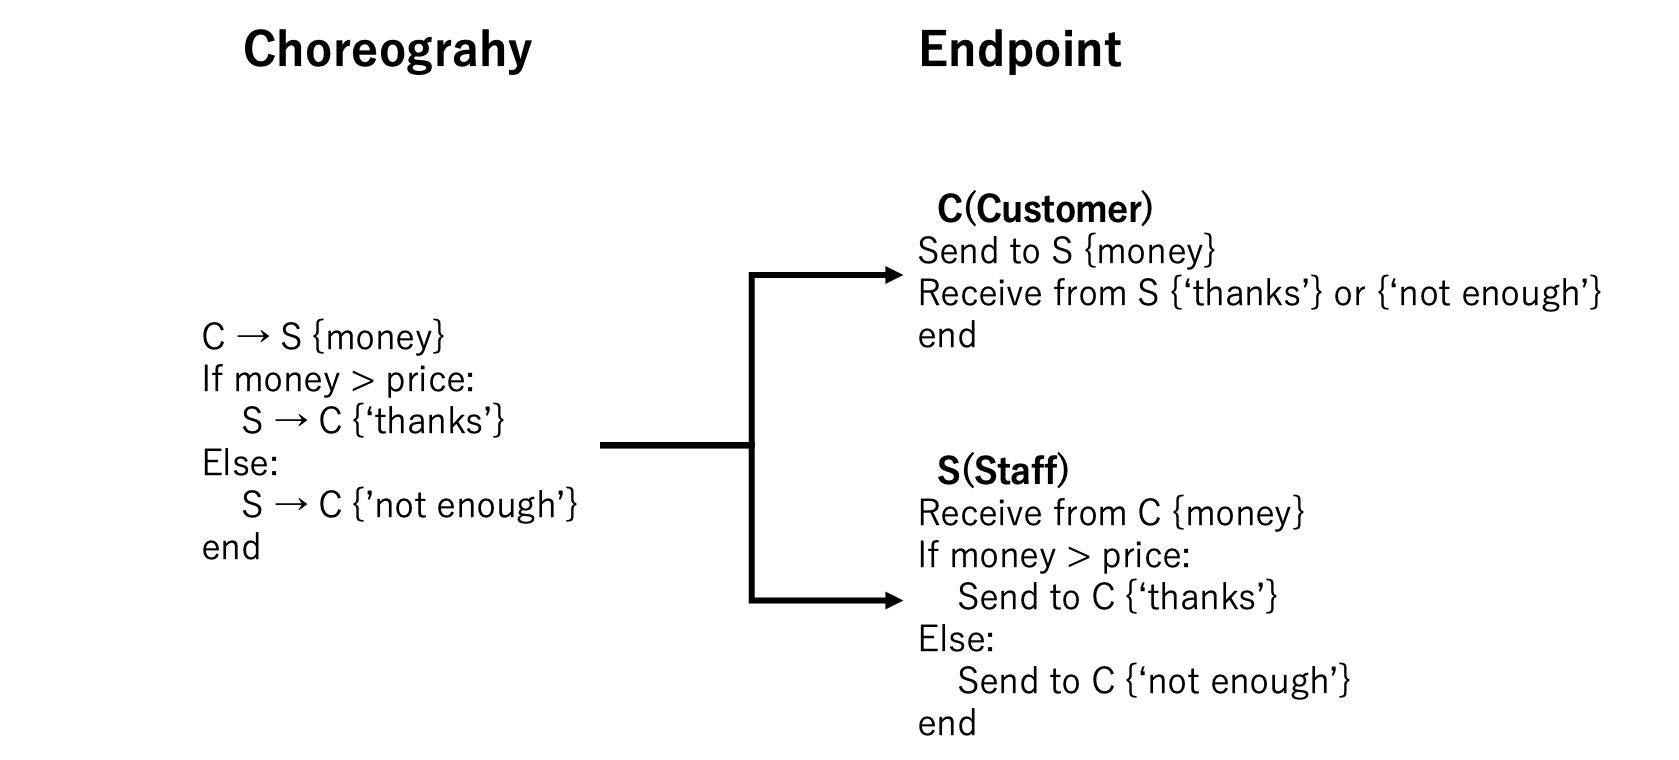
\includegraphics[scale=0.5]{image/cho.png}
  \caption{コレオグラフィとエンドポイント(CustomerとStaffとの会計時の会話)}
  \label{cho}
\end{figure}


エンドポイント射影とは,コレオグラフィから各参加者のプログラムを導出する操作である.
コレオグラフィックプログラミング言語にはコンパイラが付属しており,コンパイラはエンドポイント射影理論によって並行分散システム用の実行可能コードに変換する.

\begin{figure}[H]
  \centering
  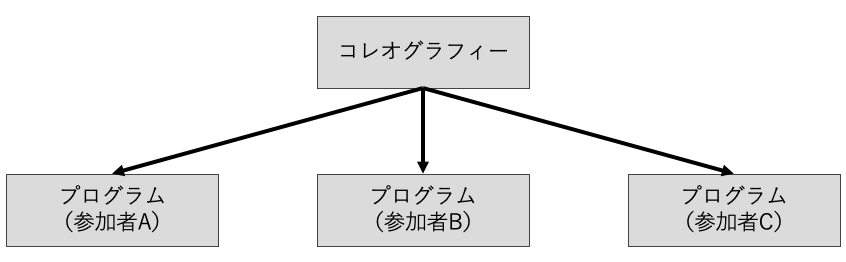
\includegraphics[scale=0.5]{image/epp.png}
  \caption{エンドポイント射影(参加者3人)}
\end{figure}
%%%%%%%%%%%%%%%%%%%%%%%%%%%%%
\subsection{Choral}
Choral\cite{choral}はJavaをベースとしたコレオグラフィックプログラミング言語である.
マルチスレッド環境で動作するプログラムでは,データ競合が発生しないようにコーディングする事がプログラマの大きな負担となっていたが,
Choralは,分散システムに従わせたいプロトコル全体を単一のプログラムとして作成できるため,これらの負担が軽減される.
Choralのオブジェクトには${\color{blue}{T@(R_1,\cdots,R_n)}}$という形式の型があり,Javaの基本的なオブジェクトインターフェイス$T$に
各参加者の情報となるパラメータ${\color{blue}{R_1,\cdots,R_n}}$が存在する.これにより,Choralプログラムをコンパイルする際に各参加者のプログラムが,
コレオグラフィに従った形で自動的に生成することができる.
%code\ref{choral}はClient,Service,IPの3つの役割からなる分散認証システムを簡約したものである.
%Choralプログラムはクラス名や変数,型などに$@$で参加者名の情報を加えている.
また,Choralにはcomメソッドとselectionメソッドなるものがある\cite{objective_Choreographies}.

\begin{lstlisting}[caption=データ転送のための基本的な有向チャンネル,label=com]
interface DiDataChannel@(A,B)<T@C> {
  <S@D extends T@D> S@B com(S@A m);
} 
\end{lstlisting}
code\ref{com}はcomメソッドの最も簡易的に使用しているインターフェースの例である.DiDataChannelは,
AとBで抽象化された2つの参加者間の有向チャンネルで,型パラメータTで抽象化された型のデータをAからBに転送するための
インターフェースである.データ転送はcomを呼び出すことによって実行される.comは,Aに位置するTのサブタイプの任意の値S@Aを取り,S@Bを返す.
%例えばcode\ref{choral}の8行目の外側のcomはClientからIPへString型のメッセージ(credentional@IP.getsalt(...))を転送することを意味する.

\begin{lstlisting}[caption=selectionメソッドの定義,label=select]
interface DiSelectChannel@(A,B) {
  @SelectionMethod
  <T@C extends Enum@C<T>> T@B select(T@A m);
} 
\end{lstlisting}
selectionメソッドは参加者間で列挙型のインスタンスを送信する際に使用する.
%例えば,code\ref{choral}の11行目,18行目ではClientからIPへ列挙型の値OK,KOを転送することを意味する.
selectionメソッドは選択を意味し,プロジェクション後はswitch文に変換されてJavaプログラムが生成される.

Choralは独自のパーサーにより,Choralプログラムからコンパイラを通して各エンドポイントのJavaプログラムが自動導出される.
それぞれのJavaプログラムはコレオグラフィに従っているため,相互関係によるバグがないことが保証されている.
これは,マルチパーティなプログラムを記述するJavaプログラマにとっては大きなメリットである.

%%%%%%%%%%%%%%%%%%%%%%%%%%%%%%%%%%%%%%%%%%%%%%%%%%
\section{Mypy}
%\begin{itemize}
%  \item MypyはPythonの静的型検査器であり,既存のPythonコードに型アノテーションを追加することで,型が誤っていると警告を出すようになる.
%  \item Pythonは動的型付け言語であるため実行時にのみエラーが表示されるが,Mypyにより実行しなくてもコンパイル時にバグが検出できる.
%  \item Mypyの仕組み(プログラム→AST→型検査→エラー)← 図でやる
%\end{itemize}
Pythonは動的型付け言語で実行時にのみエラーが表示されるので,コンパイル時に型に対するエラーは表示されない.
Mypy\cite{Mypy}はPythonの静的型検査器であり,既存のPythonコードに型アノテーションを追加することで,型が誤っていると警告を出すようになる.
これによりコンパイル時にバグの検出が可能になり,安全なコーディングが可能となる.
\begin{lstlisting}[caption=型注釈のないPythonコード]
def greeting(name):
  return 'Hello ' + name

greeting(123)
greeting(b'Alice')
\end{lstlisting}
\begin{lstlisting}[caption=型注釈のあるPythonコード]
def greeting(name: str) -> str:
  return 'Hello ' + name

greeting('World')  !# No error!
greeting(3)         
!# Argument 1 to 'greeting' has incompatible type 'int'; expected 'str'!
greeting(b'Alice')  
!# Argument 1 to 'greeting' has incompatible type 'bytes'; expected 'str'!
\end{lstlisting}
本研究ではMypyを別のPythonアプリケーションに統合するために,PythonプログラムにMypy.apiをインポートして型検査を行う.
図\ref{mypyproc}は通常のMypyを使用した際の型検査のプロセスである.
\begin{figure}[H]
  \centering
  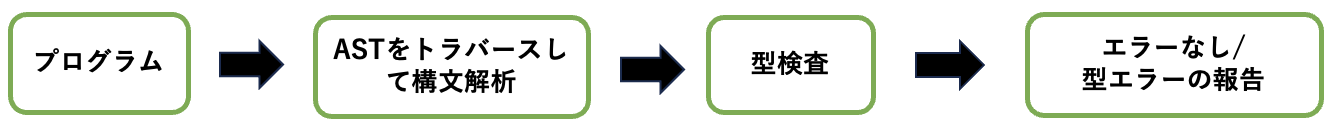
\includegraphics[scale=0.6]{image/mypyprocess.png}
  \caption{Mypyプロセス}
  \label{mypyproc}
\end{figure}

\begin{itemize}
  \item 標準的に備わっているtypeshedの話はいるのか
  \item トラバース方法について
\end{itemize}
%%%%%%%%%%%%%%%%%%%%%%%%%%%%%%%%%%%%%%%%%%%%%%%%%%
\chapter{PyChoral}
\section{PyChoralの概要}
PyChoralはPythonベースのコレオグラフィックプログラミング言語である.PyChoralでマルチパーティなプログラムを記述し,
コンパイルすることで型エラーがない場合は,各参加者のPythonプログラムコードがコレオグラフィに従った形で自動導出することができる.

PyChoralではMypyを活用した型検査のプロセスを改造し,型検査を行なった後に各エンドポイントのASTを再構築する.
射影後に再構築されるASTは新しいデータ構造を取り,それに従ったPythonプログラムが生成される(詳細は4.4.2節).

\begin{figure}[H]
  \centering
  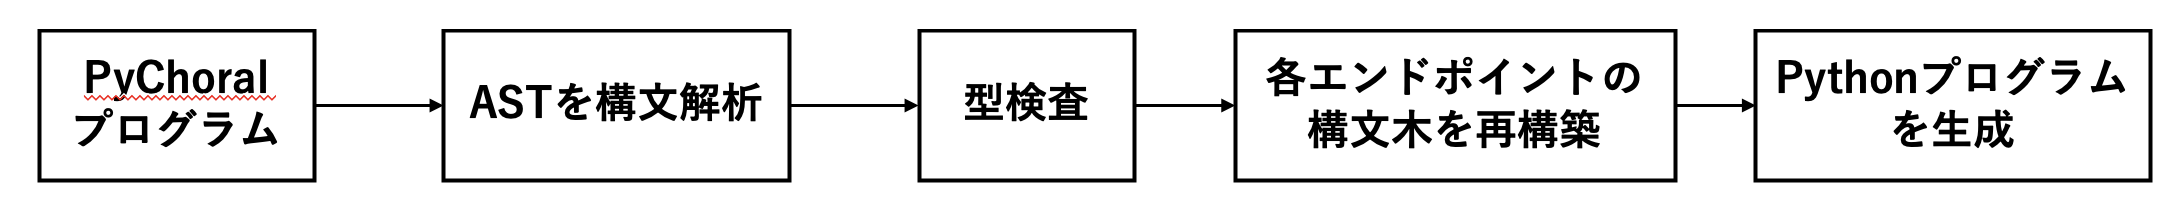
\includegraphics[scale=0.4]{image/pychoralprocess.png}
  \caption{PyChoralプロセス}
  \label{pychoralprocess}
\end{figure}

%\section{PyChoralプログラムと生成されるPythonプログラムの例}
コード\ref{pychoral}は図\ref{cho}のコレオグラフィをPyChoralで記述したプログラムである.継承クラス$\textsf{Ch2}$はクラス内で2者(ここではC,S)の振舞いが関係することを示す.
関数$\textsf{check}$の引数\texttt{price,money}の型注釈$\textsf{At[object,R]}$はその型を持つ変数の値の型と関連する参加者の情報を併せ持つ型クラスである.
\textsf{ch\_CS,ch\_SC}の型注釈$\textsf{Channel[object,R1,R2]}$は2者間のqueueを表し,転送される値,送信者,受信者の型を持つ型クラスである.
\textsf{e@R()}は参加者Rの値eであることを示す.\textsf{com}は送信者の値を受信者に転送するメソッドである.
\begin{lstlisting}[caption=PyChoral,label=pychoral]
class Check(Ch2[S,C]):
    def __init__(self):
        self.ch_CS : Channel[int,C,S] = Channel[int,C,S]('C','S')
        self.ch_SC : Channel[str,S,C] = Channel[str,S,C]('S','C')

    def check(self,price:At[int,S],money:At[int,C]) -> At[str,C]:
          payment = self.ch_CS.com(money)
          if (payment > price):
              return self.ch_SC.com('thanks'@S())
          else:
              return self.ch_SC.com('not enough'@S())
\end{lstlisting}
射影後の参加者C,Sのプログラムは射影の定義に従い,それぞれ関係ある式,文が射影されて生成される.
生成されたPythonプログラムは型注釈がない.PyChoralプログラムの型注釈において射影対象でない参加者が関連する値は消える.

\begin{lstlisting}[caption=generated Python,label=python]
# Customer
class Check_C():
    def __init__(self):
        self.ch_CS = Channel[int,C,S]('C','S')
        self.ch_SC = Channel[str,S,C]('S','C')
    def check(self,money):
        Unit.id(self.ch_CS.com(money))
        return self.ch_SC.com()

# Staff
class Check_S():
    def __init__(self):
        self.ch_CS = Channel[int,C,S]('C','S')
        self.ch_SC = Channel[str,S,C]('S','C')
    def check(self,price):
        payment = self.ch_CS.com()
        if payment>price:
            return Unit.id(self.ch_SC.com('thanks'))
        else:
            return Unit.id(self.ch_SC.com('not enough'))
\end{lstlisting}
\section{PyChoralの構文と射影定義}
この節では本研究で実装したPyChoralプログラムの構文及びコンパイル時のエンドポイント射影の定義を示す.
まず,PyChoralの構文を示し,Pythonとの違いについて述べる.次に,PyChoralプログラムからPython
プログラムが自動導出されるためのエンドポイント射影の定義を示す.

\subsection{syntax}
\begin{figure}[H]
  \centering
  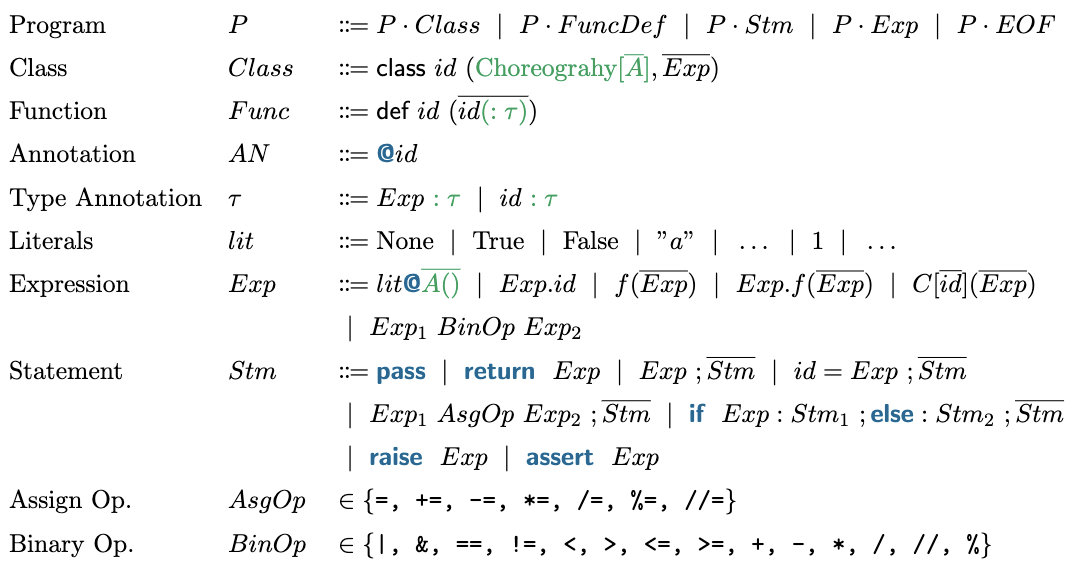
\includegraphics[scale=0.75]{image/syntax.png}
  \caption{Syntax of PyChoral}
  \label{syntax}
\end{figure}

PyChoralのクラス定義は,クラス継承の第一引数にChoreographyクラスを継承させる.
Choreographyクラスは以下のように定義され,どの参加者が関係するか分かるようなクラスとなっている.
Chクラスの引数はジェネリック型をとっており,任意の型を後から取ることができるプレースホルダーとして機能している.
継承されるChoreograhyクラスは,子クラスに関わる参加者の数によって決定される.2者(A,B)間の通信の場合はクラスCh2を継承させ,実際のPyChoralプログラムの際は$\textsf{class}~\text{Foo(Ch2[A,B])}$と記述する.
式はリテラルのみ$@$をつけて参加者の情報を得られる事とする.その他の式は基本的に型注釈もしくはMypyを活用して検査した際に取得できる型情報から参加者の情報を得る.文の構文はPythonと変化はない.

\begin{lstlisting}[caption=Choreographyクラス,label=ch]
class Ch1(Generic[_R1]):
    pass
class Ch2(Generic[_R1,_R2]):
    pass
class Ch3(Generic[_R1,_R2,_R3]):
    pass
  ... 
\end{lstlisting}


%%%%%%%%%%%%%%
\subsection{Projection}
この節ではPyChoralプログラムから各参加者のPythonプログラムを導出するために重要なエンドポイント射影の定義についていくつか示す(定義の全体は付録Aを参照).
とあるマルチスレッドプログラムの参加者$\cyan{\text{A}}$に対するPyChoralの項のプロジェクションは$\projection{Term}{A}$と記し,これは$Term$における参加者$\cyan{\text{A}}$の振舞いを表すPythonの項となる.
これは図\ref{pychoralprocess}の3ステップ目にあたる.

クラス定義の射影はクラス継承の第一引数Chクラスに存在する参加者名によってPythonの項を生成する.
\begin{alignat*}{2} 
  &\projection{\textsf{class} ~id~(Ch[\overline{\cyan{R}}],\overline{Exp}):\overline{Stm}}{A}=
  \begin{cases}
    \textsf{class} ~id\_{\cyan{A}}~(\overline{\projection{Exp}{A}}):\overline{\projection{Stm}{A}} & \text{if}~~ {\cyan{A}} \in \overline{\cyan{R}}\\
    \text{absent} & \text{if}~~ {\cyan{A}} \notin \overline{\cyan{R}}
  \end{cases}
\end{alignat*}
(例)参加者$\cyan{\text{A}},\cyan{\text{B}}$が関わるクラス$\textsf{Foo}$の射影
\begin{alignat*}{2} 
  &~~~~~~~~~\textsf{PyChoral} ~~~~~~~~~~~~~\Longrightarrow~~~~~~ \textsf{Python}\\
  &\projection{\textsf{class} ~\text{Foo} \text{(Ch2[{\cyan{A}},{\cyan{B}}])}}{A} ~~~\Longrightarrow~~~ \textsf{class} ~\text{Foo\_{\cyan{A}}}(~)\\
  &\projection{\textsf{class} ~\text{Foo} \text{(Ch2[{\cyan{A}},{\cyan{B}}])}}{B} ~~~\Longrightarrow~~~ \textsf{class} ~\text{Foo\_{\cyan{B}}}(~)\\
  &\projection{\textsf{class} ~\text{Foo} \text{(Ch2[{\cyan{A}},{\cyan{B}}])}}{C} ~~~\Longrightarrow~~~ 
\end{alignat*}

関数定義は引数の型注釈に射影される参加者の情報があればその引数を残す.
\begin{alignat*}{2} 
  &\projection{\textsf{def} ~id~(\overline{id:TE}):\overline{Stm}}{A} = \textsf{def} ~id~ (\overline{id}):\overline{\projection{Stm}{A}}\\
\end{alignat*}
(例)参加者$\cyan{\text{A}}$が関連する引数をもつ関数\text{f}の射影
%参加者$\cyan{\text{A}}$に対して関数定義$\textsf{def}~f(x:\text{At[int,{\cyan{A}}]})$から射影された関数は$\textsf{def}~f(x)$となり,$\textsf{def}~f(x:\text{At[int,{\cyan{B}}]})$から射影された関数は$\textsf{def}~f()$となる.
\begin{alignat*}{2} 
  &~~~~~~~~~~~\textsf{PyChoral} ~~~~~~~~~~~~~~~\Longrightarrow~~~~~~ \textsf{Python}\\
  &\projection{\textsf{def} ~\text{f}~(\text{self},x:\text{At[int,{\cyan{A}}]})}{A} ~~~\Longrightarrow~~~ \textsf{def} ~\text{f}~ (\text{self},x)\\
  &\projection{\textsf{def} ~\text{f}~(\text{self},x:\text{At[int,{\cyan{A}}]})}{B} ~~~\Longrightarrow~~~ \textsf{def} ~\text{f}~ (\text{self})\\
\end{alignat*}

式 Expression は射影する際に文字列を生成する($\text{Expression} \rightarrow \text{String}$).
リテラルは$@$を付けることで関係する参加者を判別可能である.射影される参加者の情報がある場合はリテラルをそのまま生成し,ない場合はUnit値が生成される.
%\begin{alignat*}{2} 
%  &\projection{lit\mblue{@}(\overline{{\color{cyan}{B}}()}):\tau}{A}=
%  \begin{cases}
%    lit & \text{if}~~ {\color{cyan}A} \in \overline{\color{cyan}{B}}\\
%    \texttt{Unit.id} &\text{otherwise}
%  \end{cases}\\
%\end{alignat*}
%(例)$123@{\cyan{\text{A}}}()$の射影
%\begin{alignat*}{2} 
%  &\projection{123\mblue{@}{\color{cyan}{A}}()}{A} = 123\\
%  &\projection{123\mblue{@}{\color{cyan}{A}}()}{B} = \texttt{Unit.id}
%\end{alignat*}
その他の式は型注釈や型推論から参加者の情報を取得し,各定義によって射影される.
例えば,メソッド呼び出し$Exp_1.f(\overline{Exp_2})$はレシーバオブジェクト$Exp_1$,引数$\overline{Exp_2}$,
メソッド呼び出し全体の型情報に射影される参加者の情報があるかどうかで場合分けをする.
ここで,$\tau$はメソッド呼び出し全体の型情報を表す.
\begin{alignat*}{2} 
  &\projection{Exp_1.f(\overline{Exp_2}):\tau}{A}=
  \begin{cases}
    \projection{Exp_1}{A}.f(\overline{\projection{Exp_2}{A}}) \\
    ~~~~~~~~~~~~~~~~~~~\text{if}~~ {\color{cyan}A} \in \text{rolesOf}(Exp_1) \wedge {\color{cyan}A} \in \text{rolesOf}(\overline{Exp_2})\\
    ~~~~~~~~~~~~~~~~~~~~~~~~~~~~~~~~~~~~~~~~~~ \wedge {\color{cyan}A} \in \text{rolesOf}(Exp_1.f(\overline{Exp_2}))\\
    \texttt{Unit.id}(\projection{Exp_1}{A}.f(\overline{\projection{Exp_2}{A}})) \\
    ~~~~~~~~~~~~~~~~~~~\text{if}~~ {\color{cyan}A} \in \text{rolesOf}(Exp_1) \wedge {\color{cyan}A} \notin \text{rolesOf}(Exp_1.f(\overline{Exp_2}))\\
    \texttt{Unit.id}(\projection{Exp_1}{A},\overline{\projection{Exp_2}{A}}) ~~~~~\text{otherwise}
  \end{cases}\\
\end{alignat*}
(例)$\cyan{\text{A}}$と$\cyan{\text{B}}$のチャネルで$\cyan{\text{A}}$から$\cyan{\text{B}}$へメッセージを送るメソッド呼び出し
%$\text{ChAB.com('msg'@{\cyan{A}}())}$を参加者$\cyan{\text{A}}$,参加者$\cyan{\text{B}}$,参加者$\cyan{\text{C}}$に対してそれぞれ射影すると,以下のようになる.
\begin{alignat*}{2} 
  &~~~~~~~~~\textsf{PyChoral} ~~~~~~~~~~~~~~~\Longrightarrow~~~~~~~~~~~~~~ \textsf{Python}\\
  &\projection{\text{ChAB.com('msg'@{\cyan{A}})}}{A} ~~~\Longrightarrow~~~ \texttt{Unit.id}(\text{ChAB.com('msg')})\\
  &\projection{\text{ChAB.com('msg'@{\cyan{A}})}}{B} ~~~\Longrightarrow~~~ \text{ChAB.com(\texttt{Unit.id})}\\
  &\projection{\text{ChAB.com('msg'@{\cyan{A}})}}{C} ~~~\Longrightarrow~~~ \texttt{Unit.id}(\texttt{Unit.id},\texttt{Unit.id})
\end{alignat*}
メソッド呼び出しの場合分けに出てくる$\textsf{rolesOf(~)}$とは,式の型情報を参照し,その型から参加者の情報を文字列の集合として返す関数である.上記の例の場合,
$\text{rolesOf}(Exp_1) = \{\text{A,B}\}$, $\text{rolesOf}(\overline{Exp_2}) = \{\text{A}\}$, $\text{rolesOf}(Exp_1.f(\overline{Exp_2})) = \{\text{B}\}$である.

文Statementは中に現れる式や文をそれぞれ射影する形式を取る.例えばreturn文の射影は$\projection{\mblue{return} ~ Exp;}{A} = \mblue{return} ~ \projection{Exp}{A}$
%\begin{alignat*}{2} 
%  &\projection{\mblue{return} ~ Exp;}{A} = \mblue{return} ~ \projection{Exp}{A}\\
%\end{alignat*}
となり,返値$Exp$の射影が反映されたreturn文が新しくPythonプログラムとして生成される.
しかし,特定の式文(expression statement)と条件文(if)は射影の形式が異なる.

式文の式($Exp$)がメソッド呼び出しであり,メソッド名が\textsf{select}の場合を選択文と呼ぶこととする.この選択文は射影するとmatch文としてPythonプログラムが生成される.
この時,メソッドの引数はEnumクラスの値であり,これがMatch文における場合分け時の値($id_2$)となる.
\begin{alignat*}{2} 
  &\projection{Exp;\overline{Stm}}{A} =
  \begin{cases}
    \mblue{match} ~\projection{Exp}{A}: \\
    ~~~~~\mblue{case} ~id_2: \projection{\overline{Stm}}{A};~~~~~ \text{if}~~Exp = Exp_1.\texttt{select}(id_1.id_2\mblue{@}{\cyan{A}}()),~ id_1.id_2:\texttt{Enum}\\ %~~~ \text{Name}(f) = \texttt{Select}\\%&~~~~ {\cyan{A}} \in \text{rolesOf}(Exp.f(\overline{Exp})) ~~\text{and}\\
    ~~~~~\mblue{case} ~\_\_: \text{assert False}; \\
    \projection{Exp}{A};\projection{\overline{Stm}}{A} ~~~~~ \text{otherwise}\\
  \end{cases}
\end{alignat*}
if文は,条件式が射影対象の参加者が関係する式であれば,そのままif文の構造をPythonプログラムで生成する.
そうでない場合はif文は消え,then節とelse節に存在する後続のStatementを正規化し,マージしたものが式(Exp)に続いた形で射影される(マージと正規化の詳細は付録Bを参照).
\begin{alignat*}{2} 
  &\projection{\mblue{if}~Exp:Stm_1~;\mblue{else}:Stm_2 ~;\overline{Stm}}{A}=\\
  &
  ~~~~~~~~~~~\begin{cases}
    \mblue{if}~\projection{Exp}{A} : \projection{Stm_1}{A} ~; \mblue{else}:\projection{Stm_2}{A} ~;\projection{\overline{Stm}}{A} & \text{if}~~ \text{rolesOf}(Exp) = \cyan{A}\\
    \projection{Exp}{A} ~; \nl{\projection{Stm_1}{A}} \mg \nl{\projection{Stm_2}{A}} ~;\projection{\overline{Stm}}{A} & \text{otherwise}
  \end{cases}\\
\end{alignat*}
マージ演算子$\mg$は,分岐のプログラムを結合する演算子である.基本的に,2つのPythonの項が与えられると再帰的にマージするには,それらがmatch文でない限りは等価であるとする.
ここではそのmatch文のマージについて述べる.
\begin{alignat*}{2} 
  & \mblue{match}~Exp: ~~~~~~~~~~~~~~~~~~~~\mblue{match}~Exp': ~~~~~~~~~~~~~~~~~~~~\mblue{match}~Exp \mg Exp':\\
  & ~~~\mblue{case}~id_a : Stm'_a; ~~~~~~~~~~~~~~~~\mblue{case}~id_a : Stm''_a; ~~~~~~~~~~~~~~~~\mblue{case}~id_a : Stm'_a \mg Stm''_a;\\
  & ~~~\cdots ~~~~~~~~~~~~~~~~~~~~~~~~~~~~~~~~~\cdots ~~~~~~~~~~~~~~~~~~~~~~~~~~~~~~~~~~\cdots\\
  & ~~~\mblue{case}~id_x : Stm'_x; ~~~~~~\mg~~~~~~\mblue{case}~id_x : Stm''_x; ~~~~~~=~~~~~~\mblue{case}~id_x : Stm'_x \mg Stm''_x;\\
  & ~~~\mblue{case}~id_y : Stm'_y; ~~~~~~~~~~~~~~~~~~~~~~~~~~~~~~~~~~~~~~~~~~~~~~~~~~~~~~\mblue{case}~id_y : Stm'_y; \\
  & ~~~~~~~~~~~~~~~~~~~~~~~~~~~~~~~~~~~~~~~~~\mblue{case}~id_z : Stm'_z;~~~~~~~~~~~~~~~~\mblue{case}~id_z : Stm'_z;\\
  & ~~~\mblue{case}~~\_\_ ~: Stm'_{ex}; ~~~~~~~~~~~~~~~\mblue{case}~~\_\_ ~: Stm''_{ex}; ~~~~~~~~~~~~~~~\mblue{case}~~\_\_ ~:Stm'_{ex} \mg Stm''_{ex};\\
\end{alignat*}
上記のように,2つのmatch文のマージは,$Exp$のマージを条件式とするmatch文となる.各caseに関して,両方に存在する各ケースは元のケース
に続く文($Stm_a,...$)をマージしたケースを得る.片方にしかないケースはマージ後のmatch文にそのまま加える.

%\begin{lstlisting}[caption=射影前のプログラム,label=1]
%if valid: #@IP
%  ch_Client_IP.select(AuthBranch.OK@IP())
%  ch_Service_IP.select(AuthBranch.OK@IP())
%  ...
%  return AuthResult[Client,Service](ch_Client_IP.com(t), ch_Service_IP.com(t))
%else:
%  ch_Client_IP.select(AuthBranch.KO@IP())
%  ch_Service_IP.select(AuthBranch.KO@IP())
%  return AuthResult[Client,Service]()
%\end{lstlisting}
%if文の射影の定義により,条件式が射影される参加者と関係ないためcode\ref{2}となり,これらがマージされてcode\ref{3}となる.
%$\projection{Exp}{A} ~; \nl{\projection{Stm_1}{A}} \mg \nl{\projection{Stm_2}{A}} ~;\projection{\overline{Stm}}{A}$の$\nl{\projection{Stm_1}{A}}$部分にあたるのがcode\ref{2}のOKの場合であり,$\nl{\projection{Stm_2}{A}}$部分にあたるのがcode\ref{2}のKOの場合である.
%\begin{lstlisting}[caption=射影後のプログラム(マージ前),label=2]
%#OK#
%match ch_Client_IP.select(Unit.id):
%  case OK:
%    return AuthResult(ch_Client_IP.com(Unit.id),Unit.id)
%  case __:
%    raise Exception
%
%# KO
%match ch_Client_IP.select(Unit.id):
%  case OK:
%    return AuthResult()
%  case __:
%    raise Exception
%  \end{lstlisting}
%\begin{lstlisting}[caption=射影後のプログラム(マージ後),label=3]
%match ch_Client_IP.select(Unit.id):
%  case OK:
%    return AuthResult(ch_Client_IP.com(Unit.id),Unit.id)
%  case OK:
%    return AuthResult()
%  case __:
%    raise Exception
%\end{lstlisting}
%また,マージされる後続のStatementはマージされる前に正規化される(詳細は付録A.3に記載).
%%%%%%%%%%%%%%%%%%%%%%%%%%%%%%%
\section{Mypyを活用したエンドポイント射影の実装}
\subsection{Mypyの改造}
PyChoralはPythonベースの言語のため,JavaベースのChoralを模倣するには静的型付け言語として扱え,コンパイル時にエラーの有無を判別したい.そのため,Mypyを活用して静的に型をつける.
ただし,Mypyで型注釈をつけらればChoralと同じように動くかというと,そうではない.

まず,ChoralはJavaのパーサーを改良し,独自のコンパイラを使用してChoralプログラムからJavaプログラムを自動導出しているが,本研究では既存のPythonパーサーをそのまま活用する.
Choralはクラス定義,インターフェース,変数,型に$\mblue{@}$で参加者の情報を加えていたが,Mypyの型検査ではこれを認識しない.
この問題に対して,本研究では主に2つの方法で各参加者の情報をとることにした.

1つ目の方法として,Mypyが型検査する際に参照する標準ライブラリのtypeshedに\textsf{At,Channel}といった新たな型クラスを追加し,変数の型注釈に参加者情報を加えられるようにした.
\textsf{At,Channel}の引数はジェネリック型をとっており,任意の型を後から取ることができるプレースホルダーとして機能している.
例えばPyChoralのプログラム例(code\ref{pychoral})の3行目にある$\texttt{price:At[int,S]}$は,変数$\text{price}$の型が$\text{int}$で参加者$\text{S(Staff)}$に関連する値ということが分かる.

2つ目の方法として,Mypyが型検査する際に参照されるobjectクラスに$\mblue{@}$のためのメソッド$\texttt{\_\_matmul\_\_}$を追加し,role.pyで各参加者に対して適用することで$\mathbf{123\mblue{@}A()}$
のように$\mblue{@}$をつけてプログラミングしてもMypyの型検査が通るようにした.
\begin{lstlisting}[caption=builtins.pyi]
class At(Generic[_T1,_T2],_T1):
  pass
class Channel(Generic[_T1,_R1,_R2]):
  ... 
  def com(self,msg:At[_T1,_R1]) -> At[_T1,_R2]:
      pass
  def select(self,msg:At[_T1,_R1]) -> At[_T1,_R2]:
      pass

class object:
  ... 
  def __matmul__(self:Self, _:_R) -> At[Self,_R]: ...
\end{lstlisting}
\begin{lstlisting}[caption=role.py]
class Role: # base class
  pass
class A(Role):
  def __matmul__(self, x): # @ を使えるようにする
      pass
\end{lstlisting}
改造したtypeshedを用いてPyChoral言語で記述したファイルはmypytest.pyによって一度ASTに変換して保存する(\texttt{result}).
mypycustomはMypy標準ファイルmain.pyを簡易的にしたファイルである.main.pyは構築したASTを保存せずに捨てていたが,mypycustomではASTを保存するように変更してある.
%mypycustomでは$\texttt{options.preserve\_ast = True}$によってASTを保存する.
この保存したASTに対して,木構造に変換し,その要素に対してプロジェクションを行う.
\begin{lstlisting}[caption=mypytest.py,label=mypytest]
filename = sys.argv[1]
pychoralfile = filename + '.py'
result : mypy.build.BuildResult | None = mypycustom.main(
    ['--show-traceback', '--custom-typeshed', './typeshed', pychoralfile])

src = result.graph[filename] 
typechecker = src.type_checker()

def get_roles(stm_list:list[mypy.nodes.Statement]) -> str:
    ... 
roles = get_roles(src.tree.defs)

for r in roles:
    pro_filename = pychoralfile.replace('.', '_' + r + '.')
    f = open(pro_filename, 'w')
    f.write('from pychoral' + str(len(roles)) + ' import *\n') 
    g = open(pro_filename, 'a')
    for stm in projection.projection_all(src.tree.defs,r,typechecker):
        data.stmt_to_string(stm,0)
        g.write(data.stmt_to_string(stm,0))
\end{lstlisting}
\texttt{filename}は射影の実行コマンドから受け取る.\texttt{src}には木構造に変換されたPyChoralプログラムが代入されており,\texttt{typechecker}は型検査器である.
\texttt{get\_roles}はPyChoralプログラム中のクラスから,Choreograhyクラスを元に関係する全ての参加者名を取得する関数である.
その後,全ての参加者に対して新たなファイルを作成し,射影した結果を各ファイルに印字していく.
\subsection{射影後のデータ構造}
Importを含む文,ブロック,クラス定義,関数定義は射影後,独自のデータ構造で生成される.
親クラス\textsf{Stmt}は抽象的な構文木であり,クラス継承を使ってASTの具体的なノードを子クラス(\textsf{Block,ClassDef,...})として定義している.
新しく定義したデータクラスはMypyに備わっている標準のデータクラスから射影定義に従って必要なパラメータのみ抽出したものである.
射影によって構築された新たなデータクラスは関数\texttt{stmt\_to\_string}によって文字列に変換される.この際に\texttt{' '*indent}によって印字されるファイルでのインデントのずれなどにも考慮する.
\begin{lstlisting}[caption=data.py,label=data]
class Stmt:
  pass

class Pass(Stmt):
  pass

class Return(Stmt):
    def __init__(self, exp:str):
        self.expr = exp
... 

def stmt_to_string(s:Stmt,indent:int) -> str:
    if isinstance(s,Pass):
            return ' '*indent + 'pass'
    elif isinstance(s,Return):
        return ' '*indent + 'return ' + s.expr
    ...
\end{lstlisting}

13,14行目に出てくる関数\texttt{isinstance()}はオブジェクトが指定されたクラスまたは型に属しているかどうかを判定するPythonの標準関数である.
本研究では,関数\texttt{isinstance()}をクラスまたは型の制限に使用している.
%%%%%%%%%%%%%%%%%
\subsection{projection\_all}
PyChoralプログラムの射影をするときはまず\textsf{projection\_all}が呼ばれる.関数\textsf{projection\_all}は
Statementのリスト\textsf{n},射影される参加者名\textsf{r},型チェッカー\textsf{tc}を引数にとり,新しいデータ構造を返す関数である.
\begin{lstlisting}[caption=projection\_all,label=pro.py]
def projection_all(n:list[Statement],r:str,tc:TypeChecker) -> list[Stmt]:
    result:list[Stmt] = []
    for node in n:
        if isinstance(node,Import) or isinstance(node,ImportFrom) or isinstance(node,ImportAll):
            result += [projection_md(node)]
        elif isinstance(node,ClassDef):
            result += [projection_class(node,r,tc)]
        elif isinstance(node,FuncDef):
            result += [projection_func(node,r,tc)]
        elif isinstance(node,Block):
            result += projection_block(node.body,r,tc)
        else:
            result += [projection_stm(node,r,tc)]
    return help_func.normalize_block(result)
\end{lstlisting}
\texttt{isinstance()}によって文(\texttt{node})の型はimport,クラス定義,関数定義,ブロック(文のリスト),文のいずれかとなり,それぞれの定義によって
射影された結果をresultに加えていく.射影された結果は最後に正規化(normalize)される.
%%%%%%%%%%%%%%%%%%
\subsection{projection\_exp}
式(Expression)の射影関数projection\_expは式\textsf{n},射影される参加者名\textsf{r},型チェッカー\textsf{tc}を引数にとり,文字列を返す関数である.
code\ref{pro_e.py}は4.3.2節で紹介したメソッド呼び出しの射影$\projection{Exp.f(\overline{Exp}):\tau}{A}$の一部である.メソッド呼び出しの形が$e.f(\overline{e})$とすると,$\textsf{Expression} \rightarrow \textsf{CallExpression}$のダウンキャストよりパラメータ$e.f$はn.calleeとなり,パラメータ$\overline{e}$はn.argsとなる.
パラメータ$e.f$を$e.f(\overline{e})$とすると,$\textsf{Expression} \rightarrow \textsf{MemberExpression}$のダウンキャストにより$e$をオブジェクト,$f$がメソッド名であると判別している.7行目ではメソッド呼び出し全体の型に射影される参加者名が含まれるか場合分けをしている.
射影される参加者が含まれている場合は射影定義に従って引数にあたる$\overline{e}$に対して射影を再び行う.全てのパラメータが文字列となれば最後に結合させて返す.

\begin{lstlisting}[caption=pro\_e.py,label=pro_e.py]
def projection_exp(n:Expression,r:str,tc:TypeChecker) -> str:
  ... 
  elif isinstance(n, CallExpr):
    ... 
    elif isinstance(n.callee, Mypy.nodes.MemberExpr):
      exp_list_i = []
      if r in help_func.rolesOf(n,tc): # R in e.f(e')
        for exp_i in n.args:
          exp_list_i.append(projection_exp(exp_i ,r,tc))
        exp_var_i = ','.join(exp_list_i)
        return projection_exp(n.callee.expr,r,tc) + '.' + n.callee.name + '(' + exp_var_i + ')'
      else:
        ... 
\end{lstlisting}

%%%%%%%%%%%%%%%%%%
\subsection{projection\_stm, projection\_block}
文(Statement)の射影関数projection\_stmは文\textsf{s},射影される参加者名\textsf{r},型チェッカー\textsf{tc}を引数にとり,\textsf{Stmt}を返す関数である.
ブロックの射影関数projection\_blockはStatementのリスト\textsf{s\_list},射影される参加者名\textsf{r},型チェッカー\textsf{tc}を引数にとり,\textsf{Stmt}のリストを返す関数である.
projection\_blockでは,分岐があるStatementと分岐がないStatementで場合分けされる.分岐がある場合は条件(4行目,4.3.2節selectを参照)を満たしたときMatch文のデータ構造として値が返される(7行目).
分岐がない場合はリストの先頭のStatementに対してprojection\_stmを呼び出し,残りはprojection\_blockで再帰的に呼び出す(11行目).
\begin{lstlisting}[caption=pro\_s.py]
def projection_block(s_list:list[Statement],r:str,tc:TypeChecker)-> list[Stmt]:
  ... 
  t = s.expr.accept(tc.expr_checker) 
    if isinstance(t,mypy.types.Instance) and 'enum' in t.type.defn.name and r in rolesOf(s.expr,tc) and isinstance(s.expr,mypy.nodes.CallExpr) and isinstance(s.expr.callee,mypy.nodes.MemberExpr) and s.expr.callee.name == 'select':
        if len(s.expr.args) == 1:
            pro_args = projection_exp(s.expr.args[0],r,tc)
            return [Match(projection_exp(s.expr,r,tc),[pro_args],[Block(projection_block(s_list[1:],r,tc))])]
        else:
          ... 
    else:
    return [projection_stm(s,r,tc)] + projection_block(s_list[1:],r,tc) 
def projection_stm(s:Statement,r:str,tc:TypeChecker) -> Stmt:
  ... 
\end{lstlisting}
%%%%%%%%%%%%%%%%%%%
\subsection{projection\_class}
クラス定義(ClassDef)の射影関数projection\_classは文\textsf{n},射影される参加者名\textsf{r},型チェッカー\textsf{tc}を引数にとり, 新しく定義したClassDefのデータ構造\textsf{ClassDef}を返す関数である.
新しいClassDefクラスmypy標準のClassDefクラスのパラメータに,参加者のパラメータ(\texttt{rolename})が加わった構造をしている.継承されるクラスのリスト(\texttt{base\_type\_vars})の先頭はCh1,Ch2,Ch3のいずれか
となっており,それぞれ参加者1,2,3者の振舞いが関係するクラスであると明示することで射影の際に\texttt{rolename}を取り出すことができる.
クラス定義の入れ子になっている部分は\texttt{defs}に該当し,これはStatementのリストである.クラス定義内に関数定義が出てくる場合は\texttt{defs}の先頭に対してprojection\_func()を呼び出す(7行目).
その他の式や文である場合はprojection\_blockを呼び出して,各Statementに対して射影を行なっていく(9行目).
\begin{lstlisting}[caption=pro\_class.py]
def projection_class(n:ClassDef,r:str,tc:TypeChecker) -> ClassDef:
  if 'Ch1' in str(n.base_type_exprs[0]) or 'Ch2' in str(n.base_type_exprs[0]) or 'Ch3' in str(n.base_type_exprs[0]) and r in str(n.base_type_exprs[0]):
      exprs:list[str] = []
      for exp in n.base_type_exprs[1:]:
          exprs += [(projection_exp(exp,r,tc))]
      if type(n.defs.body[0]) == FuncDef: 
          return ClassDef(n.name,r,exprs,projection_func(n.defs.body[0],r,tc))
      else: 
          return ClassDef(n.name,r,exprs,projection_block(n.defs.body,r,tc))
  ... 
\end{lstlisting}
%%%%%%%%%%%%%%%%%%%
\subsection{projection\_func}
関数定義(FuncDef)の射影関数projection\_funcは文\textsf{n},射影される参加者名\textsf{r},型チェッカー\textsf{tc}を引数にとり, 新しく定義したFuncDefのデータ構造\textsf{FuncDef}を返す関数である.
projection\_funcは主に引数の変数に対する処理を行う.変数の型注釈に対して射影される参加者が関係ある,例えば$\texttt{x:At[str,Client]}$といった引数をClientに対して射影する場合は変数だけを残し,型注釈は消す.
変数の型注釈に対して射影される参加者が関係ない場合は,その変数は引数のリストから削除する.関数定義後の式や文はprojection\_blockで射影を行う(8,10行目).
\begin{lstlisting}[caption=pro\_func.py]
def projection_func(n:FuncDef, r:str, tc:TypeChecker) -> FuncDef:
  args:list[str] = []
  if len(n.arguments) != 0:
      for arg in n.arguments:
          if arg.type_annotation is not None and r in str(arg.type_annotation):
              args.append(arg.variable.name)
          ... 
      return FuncDef(n.name,args,projection_block(n.body.body,r,tc))
  else:
      return FuncDef(n.name,[],projection_block(n.body.body,r,tc))
\end{lstlisting}
%%%%%%%%%%%%%%%%%%%
\subsection{projection\_md}
PyChoralプログラムのimport文はPythonプログラムへそのまま文字列として生成する.
\begin{lstlisting}[caption=pro\_md.py]
def projection_md(n:mypy.nodes.Statement) -> Stmt:
    if isinstance(n,mypy.nodes.Import):
        return Import(n.ids)
  ... 
\end{lstlisting}
%%%%%%%%%%%%%%%%%%%
\subsection{help\_function}
help\_functionはここまで紹介してきたprojectionの補助をする関数の集合である.
$\texttt{rolesOf()}$は式(\textsf{Expression})の型情報から参加者名を取り出す関数である.
$\texttt{rolesOf\_t()}$は型注釈から参加者名を取り出す関数である.
$\texttt{merge(),merge\_block()}$は2つの文あるいは文のリストをマージする関数である.
$\texttt{normalize(),normalize\_block()}$は文や文のリストを正規化する関数である.
\begin{lstlisting}[caption=help\_func.py]
def rolesOf(n:Expression, typeChecker:TypeChecker) -> list[str]:
  ... 
def rolesOf_t(n:Type | None, typeChecker:TypeChecker) -> list[str]:
  ... 
def merge_block(s1:list[Stmt],s2:list[Stmt]) -> list[Stmt]:
    merged_list:list[Stmt] = []
    for (t1,t2) in zip(s1,s2):
        merged_list.append(merge(t1,t2))
    return merged_list

def merge(s1:Stmt, s2:Stmt) -> Stmt: 
 ... 

def normalize_block(s_list:list[Stmt]) -> list[Stmt]:
  ... 
def normalize(s:Stmt) -> Stmt:
  ... 
\end{lstlisting}
%%%%%%%%%%%%%%%%%%
\chapter{PyChoralを用いたアプリケーション}
この節では実装を完成させた後,PyChoral言語を使用したプログラム例とコンパイル時に生成される各参加者のプログラムにより本研究の有用性を示す.
(クイックソート,マージソート,分散認証システム,etc)

%%%%%%%%%%%%%%%%%%%%%%%%%%%%%%%%%%%%%%%%%%%%%%%%%%
%\chapter{関連研究}
%%%%%%%%%%%%%%%%%%%%%%%%%%%%%%%%%%%%%%%%%%%%%%%%%%
\chapter{まとめ,今後の課題}
本研究はPythonを拡張したコレオグラフィックプログラミング言語PyChoralを実装した.
PyChoralプログラムは本研究におけるエンドポイント射影の定義によって各参加者のPythonプログラムが生成される.
エンドポイント射影理論によりPyChoralプログラム中の式は文字列として,その他は抽象クラス\textsf{Stmt}を親クラスとした新しいデータ構造として射影される.
生成された各参加者のPythonプログラムはコレオグラフィに従っているため,デッドロック等の並行性に起因するエラーが生じないことが保証されている.これにより,
マルチスレッド環境におけるプログラムが単一の言語で記述されるプログラムによって実装可能となり,Pythonでマルチスレッドプログラムをコーディングするプログラマ
の手助けとなる.

今後の課題としては以下の点がある.
\begin{itemize}
  \item 実装の完成
  
  現段階ではPyChoralプログラムをmypytestでコンパイルした時に結果としてターミナルに特定の参加者の
  Pythonプログラムが文字列として出力されるが,最終的には各参加者のPythonプログラムファイルが新たに生成されるようにする.また,記述したコードのバグを修正する.
  \item 実装したコンパイラによるPyChoralプログラムを制作する(4.5節)
    
\end{itemize}


%%%%%%%%%%%%%%%%%%%%%%%%%%%%%%
%\section*{謝辞}


%%%%%%%%%%%%%%%%%%%%%%%%%%%%%%%%%%%%%%%%%%%%%%%%%%
%参考文献
\bibliography{reference.bib}
%%%%%%%%%%%%%%%%%%%%%%%%%%%%%%%%%%%%%%%%%%%%%%%%%%%%
\appendix

\chapter{Definition of Projection, Merging, Normalizer}
\section{Projection to Python}

\begin{alignat*}{2}
  %%% ClassDef %%%
  &(Class)~~~ &&\projection{\textsf{class} ~id~(Ch[\overline{\cyan{B}}],\overline{Exp}):\overline{Stm}}{A}=
  \begin{cases}
    \textsf{class} ~id\_{\cyan{A}}~(\overline{\projection{Exp}{A}}):\overline{\projection{Stm}{A}} & \text{if}~~ {\cyan{A}} \in \overline{\cyan{B}}\\
    \text{absent} & \text{if}~~ {\cyan{A}} \notin \overline{\cyan{B}}
  \end{cases}\\
  \\
  %%% FuncDef %%%
  &(Func)~~~ &&\projection{\textsf{def} ~id~(\overline{id:TE}):\overline{Stm}}{A} = \textsf{def} ~id~ (\overline{id}):\overline{\projection{Stm}{A}}\\
  \\
  %%% Expression %%%
  % Literal
  &(Exp)~~~ &&\projection{lit\mblue{@}(\overline{{\color{cyan}{B}}()}):\tau}{A}=
  \begin{cases}
    lit & \text{if}~~ {\color{cyan}A} \in \overline{\color{cyan}{B}}\\
    \texttt{Unit.id} &\text{otherwise}
  \end{cases}\\
  %field
  &&&\projection{Exp.id:\tau}{A}=
  \begin{cases}
    \projection{Exp}{A}.id &\text{if}~~{\color{cyan}A} \in \text{rolesOf} (Exp.id)\\
    \text{absent} &\text{otherwise}
  \end{cases}\\
  %function
  &&&\projection{f(\overline{Exp}):\tau}{A} =
  \begin{cases}
    f(\overline{\projection{Exp}{A}}) &\text{if}~~ {\color{cyan}A} \in \text{rolesOf} (f(\overline{Exp}))\\
    \texttt{Unit.id}(f(\overline{\projection{Exp}{A}})) &\text{if}~~ {\color{cyan}A} \in \text{rolesOf}(\overline{Exp}) \wedge {\color{cyan}A} \notin \text{rolesOf} (f(\overline{Exp}))\\
    \texttt{Unit.id}(\overline{\projection{Exp}{A}}) &\text{otherwise}
  \end{cases}\\
  %method
  &&&\projection{Exp.f(\overline{Exp}):\tau}{A}=
  \begin{cases}
    \projection{Exp}{A}.f(\overline{\projection{Exp}{A}}) \\
    ~~~~~~~\text{if}~~ {\color{cyan}A} \in \text{rolesOf}(Exp) \wedge {\color{cyan}A} \in \text{rolesOf}(\overline{Exp})\\
    ~~~~~~~~~~~~~~~~~~~~~~~~~~~~~~~~ \wedge {\color{cyan}A} \in \text{rolesOf}(Exp.f(\overline{Exp}))\\
    \texttt{Unit.id}(\projection{Exp}{A}.f(\overline{\projection{Exp}{A}})) \\
    ~~~~~~~\text{if}~~ {\color{cyan}A} \in \text{rolesOf}(Exp) \wedge {\color{cyan}A} \notin \text{rolesOf}(Exp.f(\overline{Exp}))\\
    \texttt{Unit.id}(\projection{Exp}{A},\overline{\projection{Exp}{A}}) ~~~~~\text{otherwise}
  \end{cases}\\
  %create object
  &&&\projection{C[\overline{\color{cyan}B}](\overline{Exp}):\tau}{A}=
  \begin{cases}
    \projection{C[\overline{\color{cyan}B}]}{A} (\overline{\projection{Exp}{A}}) & {\color{cyan}A} \in \overline{\color{cyan}B}\\
    \texttt{Unit.id}(\overline{\projection{Exp}{A}}) &\text{otherwise}
  \end{cases}\\
  % binary operator
  &&&\projection{Exp_1 ~BinOp~ Exp_2}{A} = \projection{Exp_1}{A} ~BinOp~ \projection{Exp_2}{A}\\
  %role
  &&&\text{rolesOf}(\_:\tau\mblue{@}(\overline{\color{cyan}B})) = {\overline{\color{cyan}B}}\\
  &&&\text{rolesOf}(\overline{Exp}) = \bigcup_i \text{rolesOf}(Exp_i) \\
  &&&\projection{\overline{Exp}}{A} = Exp'_1,Exp'_2,\cdots,Exp'_n ~~\text{where}~~ Exp'_i = \projection{Exp_i}{A}\\ 
  \\
  \\ 
  %%% Statement %%%
  %pass
  &(Stm)~~~ &&\projection{\mblue{pass}}{A} = \mblue{pass}\\
  %return
  &&&\projection{\mblue{return} ~ Exp;}{A} = \mblue{return} ~ \projection{Exp}{A}\\
  % e;s
  &&&\projection{Exp;\overline{Stm}}{A} =
  \begin{cases}
    \mblue{match} ~\projection{Exp}{A}: \\
    ~~~~~\mblue{case} ~id_2: \projection{\overline{Stm}}{A};~~~~~ \text{if}~~Exp = Exp'.\texttt{select}(id_1\mblue{@}{\cyan{A}}.id_2):\texttt{Enum}\mblue{@}{\cyan{A}}\\ %~~~ \text{Name}(f) = \texttt{Select}\\%&~~~~ {\cyan{A}} \in \text{rolesOf}(Exp.f(\overline{Exp})) ~~\text{and}\\
    ~~~~~\mblue{case} ~\_\_: \text{assert False}; \\
    \projection{Exp}{A};\projection{\overline{Stm}}{A} ~~~~~ \text{otherwise}\\
  \end{cases}\\
  % Assignment 
  &&& \projection{id:TE = Exp~;\overline{Stm}}{A} =
  \begin{cases}
    id = \projection{Exp}{A};\projection{\overline{Stm}}{A} & \text{if}~~ {\color{cyan}A} \in \text{rolesOf}(TE)\\
    \projection{Exp}{A};\projection{\overline{Stm}}{A} & \text{otherwise}
  \end{cases}\\
  % OpAssignment
  &&& \projection{Exp_1 ~AsgOp~ Exp_2 ~; \overline{Stm}}{A} = \projection{Exp_1}{A} AsgOp~ \projection{Exp_2}{A} ~; \projection{\overline{Stm}}{A} \\
  % If
  &&&\projection{\mblue{if}~Exp:Stm_1~;\mblue{else}:Stm_2 ~;\overline{Stm}}{A}=\\
  &&&
  \begin{cases}
    \mblue{if}~\projection{Exp}{A} : \projection{Stm_1}{A} ~; \mblue{else}:\projection{Stm_2}{A} ~;\projection{\overline{Stm}}{A} & \text{if}~~ \text{rolesOf}(Exp) = \cyan{A}\\
    \projection{Exp}{A} ~; \nl{\projection{Stm_1}{A}} \mg \nl{\projection{Stm_2}{A}} ~;\projection{\overline{Stm}}{A} & \text{otherwise}
  \end{cases}\\
  % raise
  &&&\projection{\mblue{raise}~Exp}{A} = \mblue{raise}~\projection{Exp}{A}\\
  % assert
  &&&\projection{\mblue{assert}~Exp}{A} = \mblue{assert}~\projection{Exp}{A}\\
  % block
  &&&\projection{\overline{Stm}}{A} = Stm'_1,Stm'_2,\cdots,Stm'_n ~~\text{where}~~ Stm'_i = \projection{Stm_i}{A}\\  
\end{alignat*}

\section{Merging}
\begin{align*}
  % Statement
  & \text{Statement}\\
  % stm_list
  & \overset{\color{red}.}{\mg} \overline{Stm} = \overset{\color{red}.}{\mg}(Stm_1, \cdots ,Stm_n) = \nl{Stm_1} \mg \cdots \mg \nl{Stm_n}\\
  % return
  & \mblue{return}~Exp \mg \mblue{return}~Exp' = \mblue{return}~Exp \mg Exp'\\
  % raise
  & \mblue{raise}~ Exp \mg \mblue{raise}~ Exp' = \mblue{raise}~ Exp \mg Exp'\\
  % assignment op
  & (Exp_1 ~AsgOp~ Exp_2 ; \overline{Stm}) \mg (Exp'_1 ~AsgOp~ Exp'_2 ; \overline{Stm'})\\
  & ~~~~~~~ = (Exp_1 \mg Exp'_1) ~AsgOp~ (Exp_2 \mg Exp'_2) ; (\overline{Stm} \mg \overline{Stm'})\\
  % expression stmt
  & (Exp ; \overline{Stm}) \mg (Exp' ; \overline{Stm'}) = (Exp \mg Exp') ; (\overline{Stm} \mg \overline{Stm'})\\
  % if 
  \\
  & \mblue{if}~Exp_1: ~~~~~~~~~~~~~~~~~~~~\mblue{if}~Exp'_1: ~~~~~~~~~~~~~~~~~~~~\mblue{if}~Exp_1 \mg Exp'_1:\\
  & ~~~~~~Stm_1; ~~~~~~~~~~~~~~~~~~~~~~~~~ Stm'_1 ~~~~~~~~~~~~~~~~~~~~~~~~~~~ Stm_1 \mg Stm'_1\\
  & \cdots ~~~~~~~~~~~~~~~~~~~~~~~~~~~\cdots ~~~~~~~~~~~~~~~~~~~~~~~~~~~~\cdots\\
  & \mblue{elif}~Exp_n: ~~~~~~\mg~~~~~~~\mblue{elif}~Exp'_n: ~~~~~~~=~~~~~~~\mblue{elif}~Exp_n \mg Exp'_n:\\
  & ~~~~~~Stm_n; ~~~~~~~~~~~~~~~~~~~~~~~~~~ Stm'_n ~~~~~~~~~~~~~~~~~~~~~~~~~~ Stm_n \mg Stm'_n\\
  & \mblue{else}:~~~~~~~~~~~~~~~~~~~~~~~~\mblue{else}:~~~~~~~~~~~~~~~~~~~~~~~~~\mblue{else}:~\\
  & ~~~~~~Stm_e; ~~~~~~~~~~~~~~~~~~~~~~~~~~ Stm'_e ~~~~~~~~~~~~~~~~~~~~~~~~~~~ Stm_e \mg Stm'_e\\
  & \overline{Stm} ~~~~~~~~~~~~~~~~~~~~~~~~~~ \overline{Stm'} ~~~~~~~~~~~~~~~~~~~~~~~~~~ \overline{Stm} \mg \overline{Stm'}\\
  \\
  % match
  & \mblue{match}~Exp: ~~~~~~~~~~~~~~~~~~~~\mblue{match}~Exp': ~~~~~~~~~~~~~~~~~~~~\mblue{match}~Exp \mg Exp':\\
  & ~~~\mblue{case}~id_a : Stm'_a; ~~~~~~~~~~~~~~~~\mblue{case}~id_a : Stm''_a; ~~~~~~~~~~~~~~~~\mblue{case}~id_a : Stm'_a \mg Stm''_a;\\
  & ~~~\cdots ~~~~~~~~~~~~~~~~~~~~~~~~~~~~~~~~~\cdots ~~~~~~~~~~~~~~~~~~~~~~~~~~~~~~~~~~\cdots\\
  & ~~~\mblue{case}~id_x : Stm'_x; ~~~~~~\mg~~~~~~\mblue{case}~id_x : Stm''_x; ~~~~~~=~~~~~~\mblue{case}~id_x : Stm'_x \mg Stm''_x;\\
  & ~~~\mblue{case}~id_y : Stm'_y; ~~~~~~~~~~~~~~~~~~~~~~~~~~~~~~~~~~~~~~~~~~~~~~~~~~~~~~\mblue{case}~id_y : Stm'_y; \\
  & ~~~~~~~~~~~~~~~~~~~~~~~~~~~~~~~~~~~~~~~~~\mblue{case}~id_z : Stm'_z;~~~~~~~~~~~~~~~~\mblue{case}~id_z : Stm'_z;\\
  & ~~~\mblue{case}~~\_\_ ~: Stm'_{ex}; ~~~~~~~~~~~~~~~\mblue{case}~~\_\_ ~: Stm''_{ex}; ~~~~~~~~~~~~~~~\mblue{case}~~\_\_ ~:Stm'_{ex} \mg Stm''_{ex};\\
  & \overline{Stm} ~~~~~~~~~~~~~~~~~~~~~~~~~~~~~~~~~ \overline{Stm'} ~~~~~~~~~~~~~~~~~~~~~~~~~~~~~~~ \overline{Stm} \mg \overline{Stm'}\\
  \\
  & \overline{Stm} \mg \overline{Stm'} = Stm_1 \mg Stm_1'~,~Stm_2 \mg Stm_2'~,~\cdots~,Stm_n \mg Stm'_n\\
  \\
  % Expression
  & \text{Expression}\\
  & Exp \mg Exp' =
  \begin{cases}
    Exp & \text{if}~ Exp = Exp'\\
    \text{error} & \text{if}~ Exp \neq Exp'
  \end{cases}\\
\end{align*}

\section{normalizer}
\begin{align*}
  % Statement
  & \text{Statements}\\
  & \nl{\mblue{pass}} = \mblue{pass}\\
  & \nl{\mblue{return}~Exp} = \mblue{return} ~ \nl{Exp}\\
  & {\scriptsize{\text{\color{Purple}NOOP}}}(Exp) = 
  \begin{cases}
    [blank] & \text{if}~~ Exp \in \{\texttt{Unit.id, None}\}\\
    Exp & \text{otherwise}
  \end{cases}\\
  & \nl{Exp_1 ~AsgOp~ Exp_2 ; \overline{Stm}} = 
  \begin{cases}
    \nl{Exp_1} ; \nl{\overline{Stm}} & \text{if}~~ {\scriptsize{\text{\color{Purple}NOOP}}}(\nl{Exp_2}) = [blank]\\
    \nl{Exp_2} ; \nl{\overline{Stm}} & \text{if}~~ {\scriptsize{\text{\color{Purple}NOOP}}}(\nl{Exp_1}) = [blank]\\
    \nl{\overline{Stm}} & \text{if}~~ {\scriptsize{\text{\color{Purple}NOOP}}}(\nl{Exp_1},\nl{Exp_2}) = [blank]\\
    \nl{Exp_1} AsgOp \nl{Exp_2} ; \nl{\overline{Stm}} & \text{otherwise}
  \end{cases}\\
  & \nl{Exp;\overline{Stm}} =
  \begin{cases}
    \nl{\overline{Stm}} & \text{if}~~ {\scriptsize{\text{\color{Purple}NOOP}}}(\nl{Exp}) = [blank]\\
    \nl{Exp} ; \nl{\overline{Stm}} & \text{otherwise}
  \end{cases}\\
  % Expression
  & \text{Expressions}\\
  & \nl{None} = None ~~~ \nl{id} = id 
\end{align*}
\end{document}